\documentclass[../Supercritical_fluid_extraction_of_essential_oil_from_chamomile.tex]{subfiles}
\graphicspath{{\subfix{../Figures/}}}
\begin{document}
	
	\label{CH: Results}
	
	The parameter estimation problem was solved multiple time for different initial guesses. Each time-series was fitted to the model separately. First, the model with linear extraction kinetic only was fitted to the dataset. The Figure show the result of parameter estimation for dataset 1, which corresponds to the following operating conditions: 313 K, 100 bar and 6.57$\times 10^{-5}$ kg/s.
	
	\begin{figure}[!h]
		\centering
		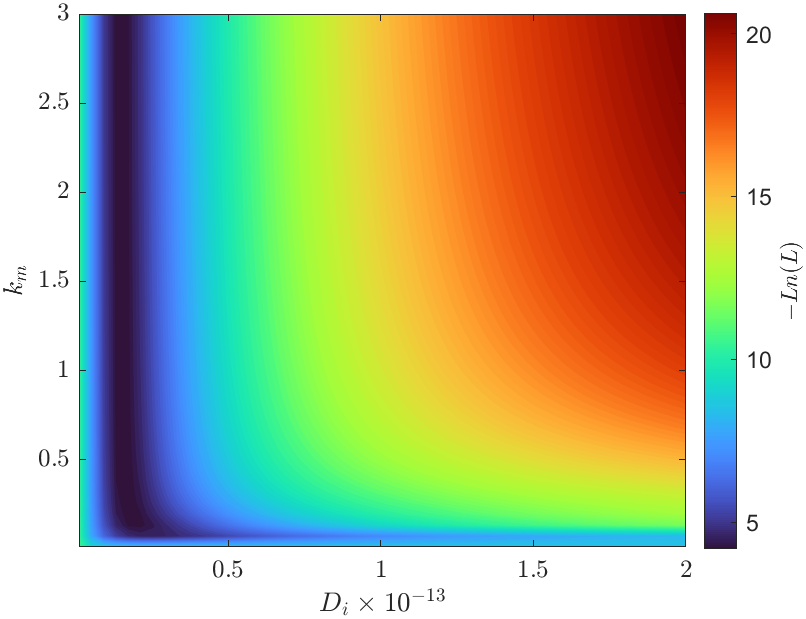
\includegraphics[trim = 0.0cm 0.0cm 0.0cm 0.0cm,clip, width=\columnwidth]{/Results_estimation/Parameter_Space_Linear_Dataset_1.png}
		\caption{Parameter space for the linear extraction kinetic model and the experiment 1}
		\label{fig: Fit_1_linear}
	\end{figure}
	
	In case of the linear kinetic two parameter are unknown, namely partition coefficient $k_m$ and the internal diffusion coefficient $D_i$. Figure \ref{fig: Fit_1_linear} shows the parameter space and corresponding values of the cost function. As the cost function is to be minimized, the lowest value of $-\ln(L)$ indicate the best fit. A black stripe around $D_i \approx 0.2)$ can be observed. That stripe indicate existence of optimal value of the $D_i$. In direction of $k_m$, the cost function is almost flat, which suggest that any value of $k_m$ above approximately 0.1 is equally good for fitting. If $k_m$ can be arbitrary point, then it can grow to the infinity. The optimizer found optimal values of the partition factors at relatively high levels. Such a behaviour suggest that the solvent is far from the saturation, and the model can be simplified. The model reduction can be introduced by considering the limit of $k_m$ in the extraction kinetic term: 
	
	{\footnotesize
		\begin{equation*}
			\begin{split}
				&\lim_{k_m \rightarrow \infty} \left({\color{black}{\color{black} c_s} }(t,z)  - \cfrac{{\color{black}\rho_s}}{{\color{black}k_m}({\color{black}T}(t,z)){\color{black}\rho}({\color{black}T}(t,z),{\color{black}P}(t))}  {\color{black}c_f}(t,z) \right)  = \\
				&= \left({\color{black}{\color{black} c_s} }(t,z)  - \cfrac{{\color{black}\rho_s}}{\infty{\color{black}\rho}({\color{black}T}(t,z),{\color{black}P}(t))}  {\color{black}c_f}(t,z) \right) = \left({\color{black}{\color{black} c_s} }(t,z) - 0 \right)
			\end{split}
	\end{equation*} }
	
	The extraction model can be modified to account for the reduced kinetic term and the axial diffusion. In such a configuration just two parameters are unknown, namely internal diffusion coefficient $D_i$ and axial diffusion coefficient $D_e^M$. Figure \ref{fig: Fit_1_Di_Dx} shows the parameter space and corresponding values of the cost function.
	
	\begin{figure}[!h]
		\centering
		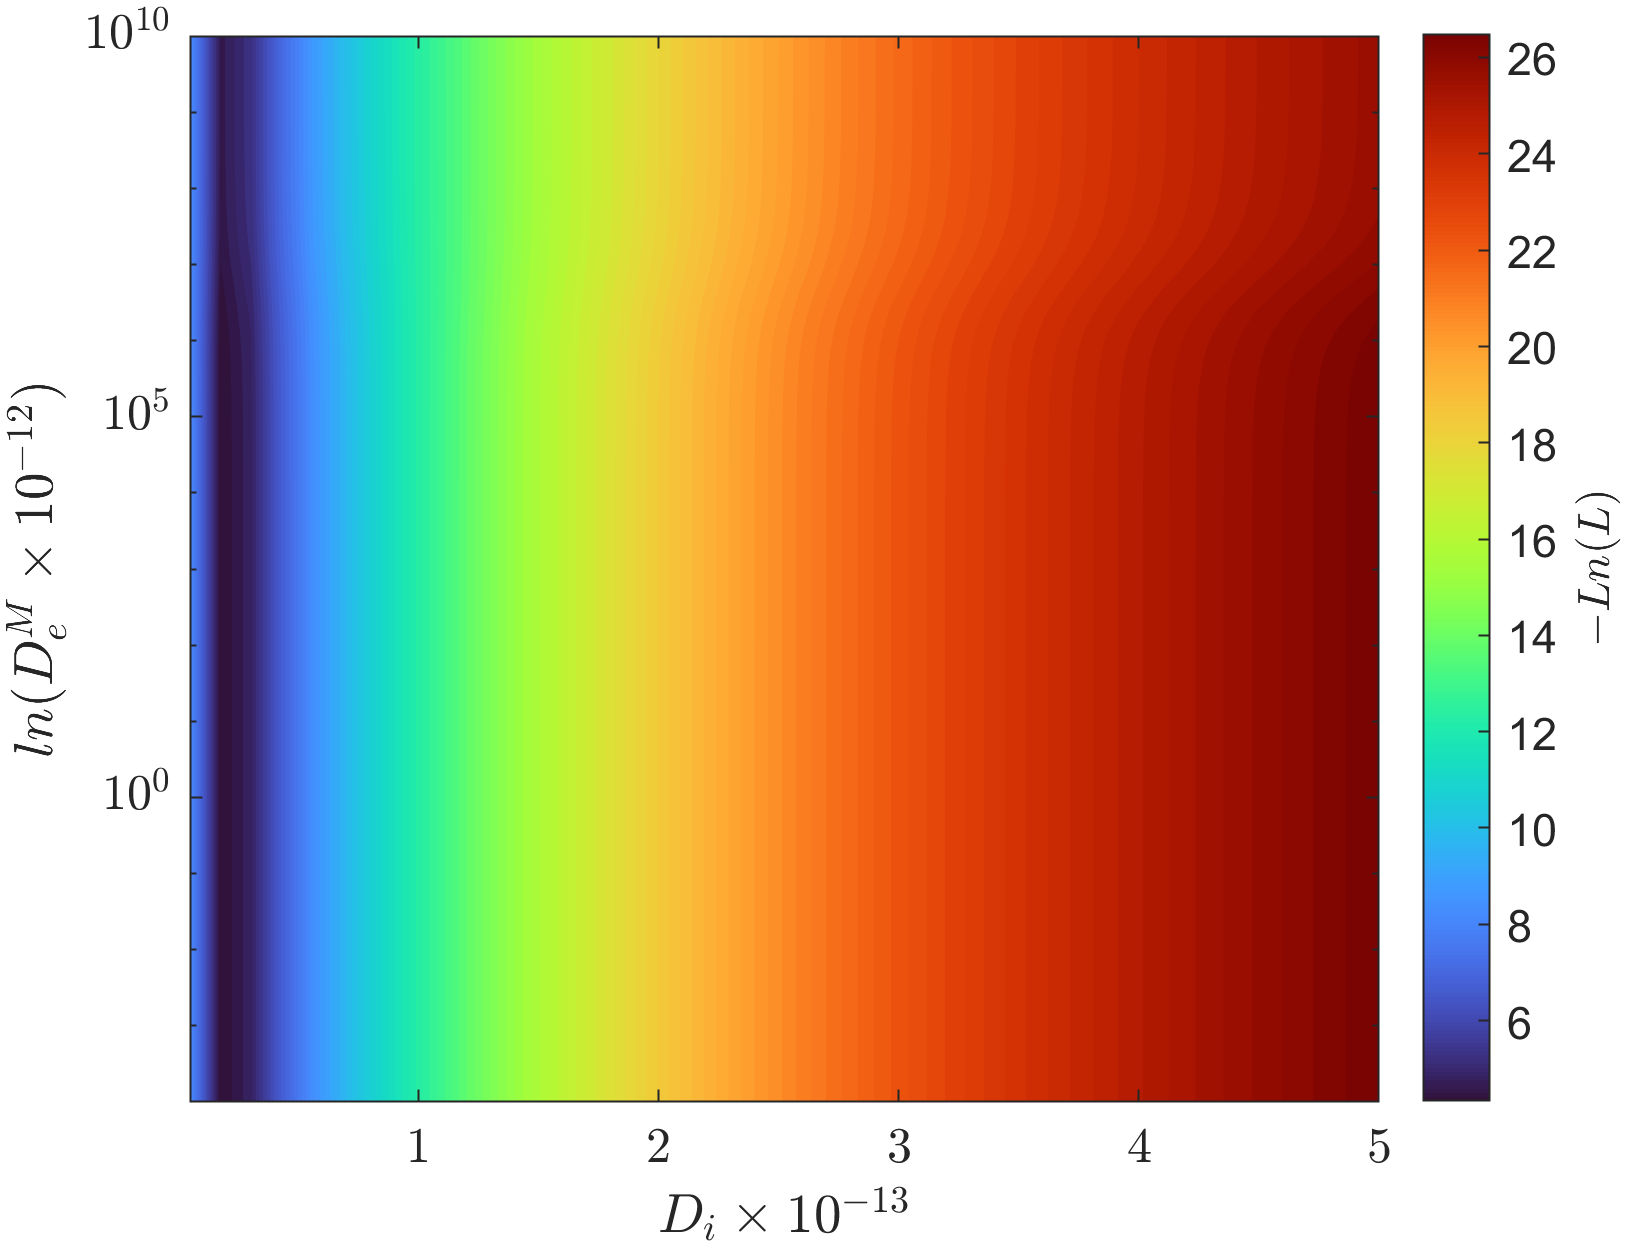
\includegraphics[trim = 0.0cm 0.0cm 0.0cm 0.0cm,clip, width=\columnwidth]{/Results_estimation/Parameter_Space_Di_Dx_Dataset_1.png}
		\caption{Parameter space for the reduced linear extraction kinetic model with and the experiment 1}
		\label{fig: Fit_1_Di_Dx}
	\end{figure}
	
	Similarly to the previous case, the optimal value of $D_i$ exist, but a unique value for the $D_e^M$ cannot be determined. A little influence of the axial diffusion coefficient can be observed on Figure \ref{fig: Fit_1_Di_Dx} in a width range of values. By selecting $D_e^M$ such it has a low value, the axial diffusion term can be reduced and removed from the model without lost of generality. The model reduction is in agreement with the work of \citet{Rahimi2011}, who worked with the same dataset and obtained Peclet numbers in the range from 290 to 400. Such a high values if Pe suggest that the advection term dominates the mass transfer and the axial diffusion is negligible.
	
	I both cases discussed above, none of the results of the fitting was not sufficient due to high or to low extraction kinetic. Following the idea behind the Broken-and-Intact and Shrinking Core models (presented in Chapter \ref{CH: Gamma_Function}), the gamma function is introduced to account for the decaying extraction kinetic. The proposed correction factor is combined with the reduced linear model, which leads to a two-parameter ($D_i^R$ and $\Upsilon$) defined by Equation \ref{Model_kinetic}. The Figure \ref{fig: Fit_1_Di_Dx} shows the parameter space with and the corresponding values of the cost function.
	
	\begin{figure}[!h]
		\centering
		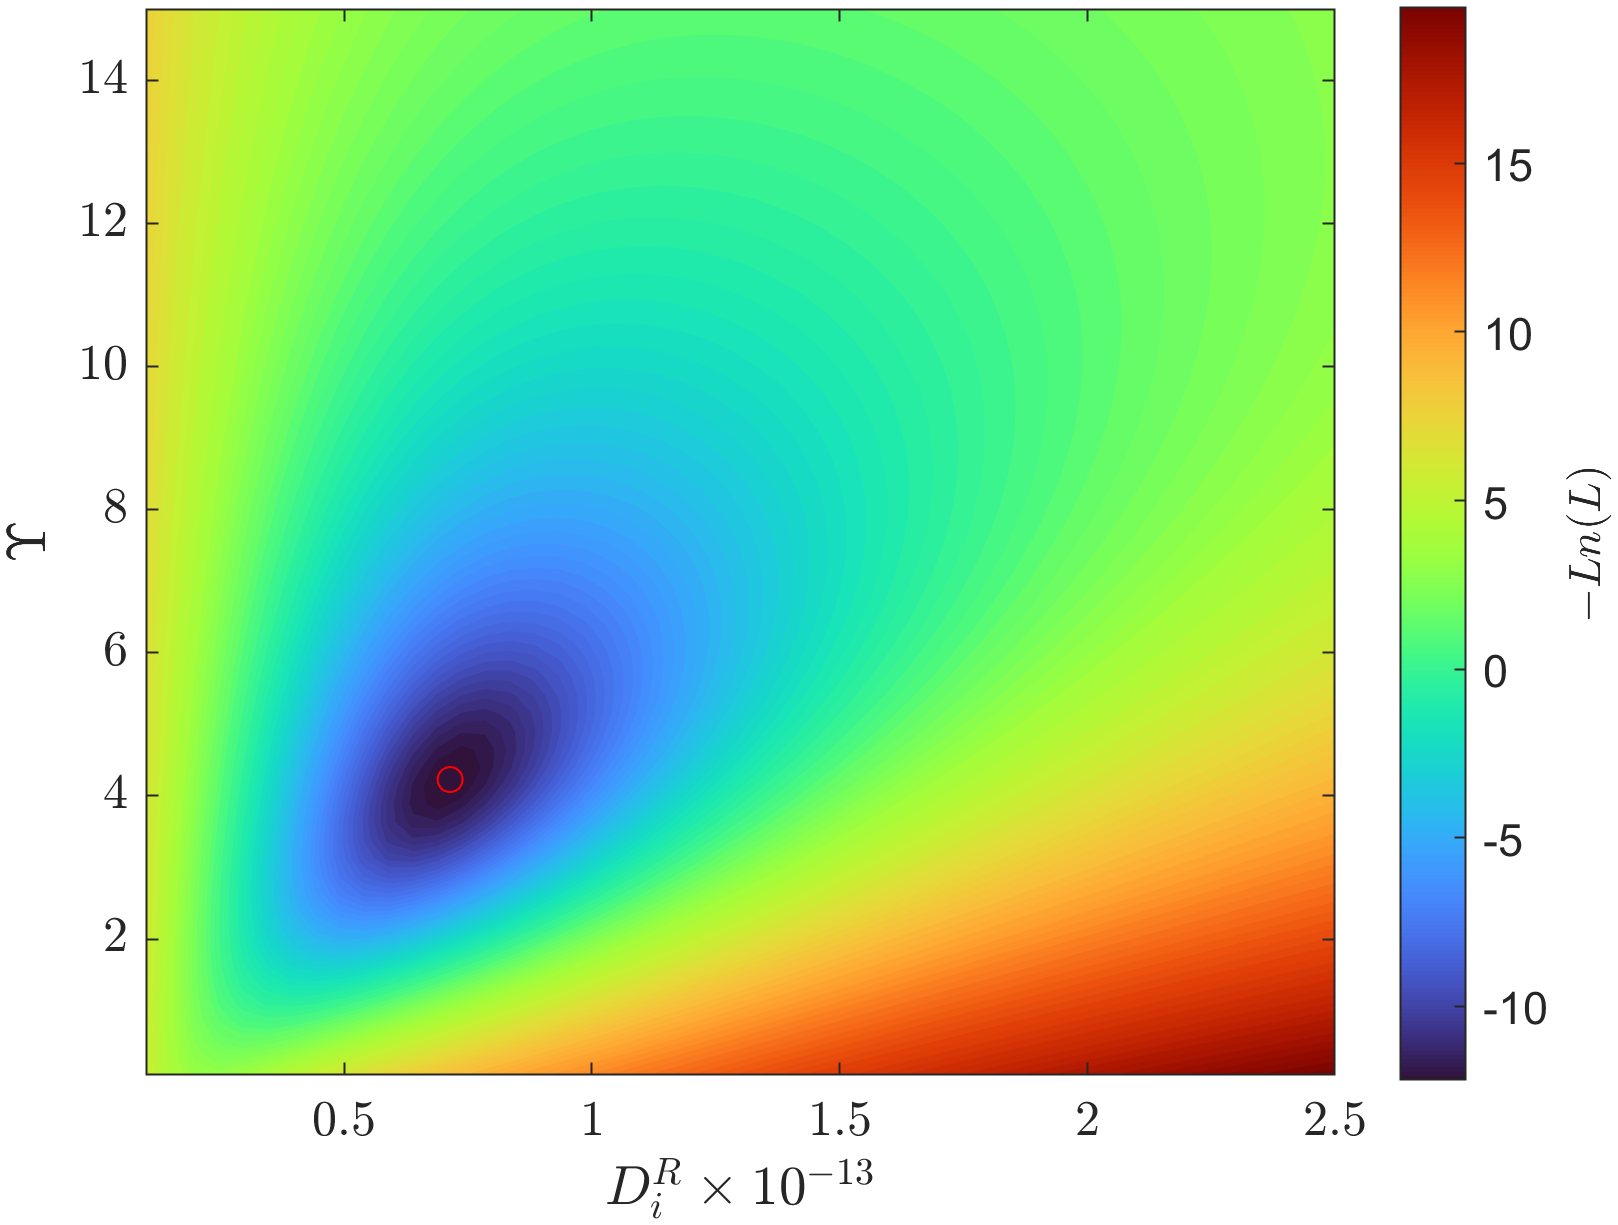
\includegraphics[trim = 0.0cm 0.0cm 0.0cm 0.0cm,clip, width=\columnwidth]{/Results_estimation/Parameter_space_Di_Gamma_dataset_1_org.png}
		\caption{Parameter space for the modified extraction model and experiment 1}
		\label{fig: Fit_1_Di_Gamma}
	\end{figure}
	
	The parameter space of the modified model is characterized by the unique minimum value, which corresponds to the solution of the parameter estimation problem for the experiment 1. The red circle shows the minimum value of the cost function found by the optimizer. The remaining experiments are fitted to the modified extraction model and results are presented in Figure \ref{fig: Fit_Di_Gamma}. The obtained results show good agreement for almost all the experiments. 

	\begin{figure}
		\centering
		\begin{subfigure}[b]{\columnwidth}
			\centering
			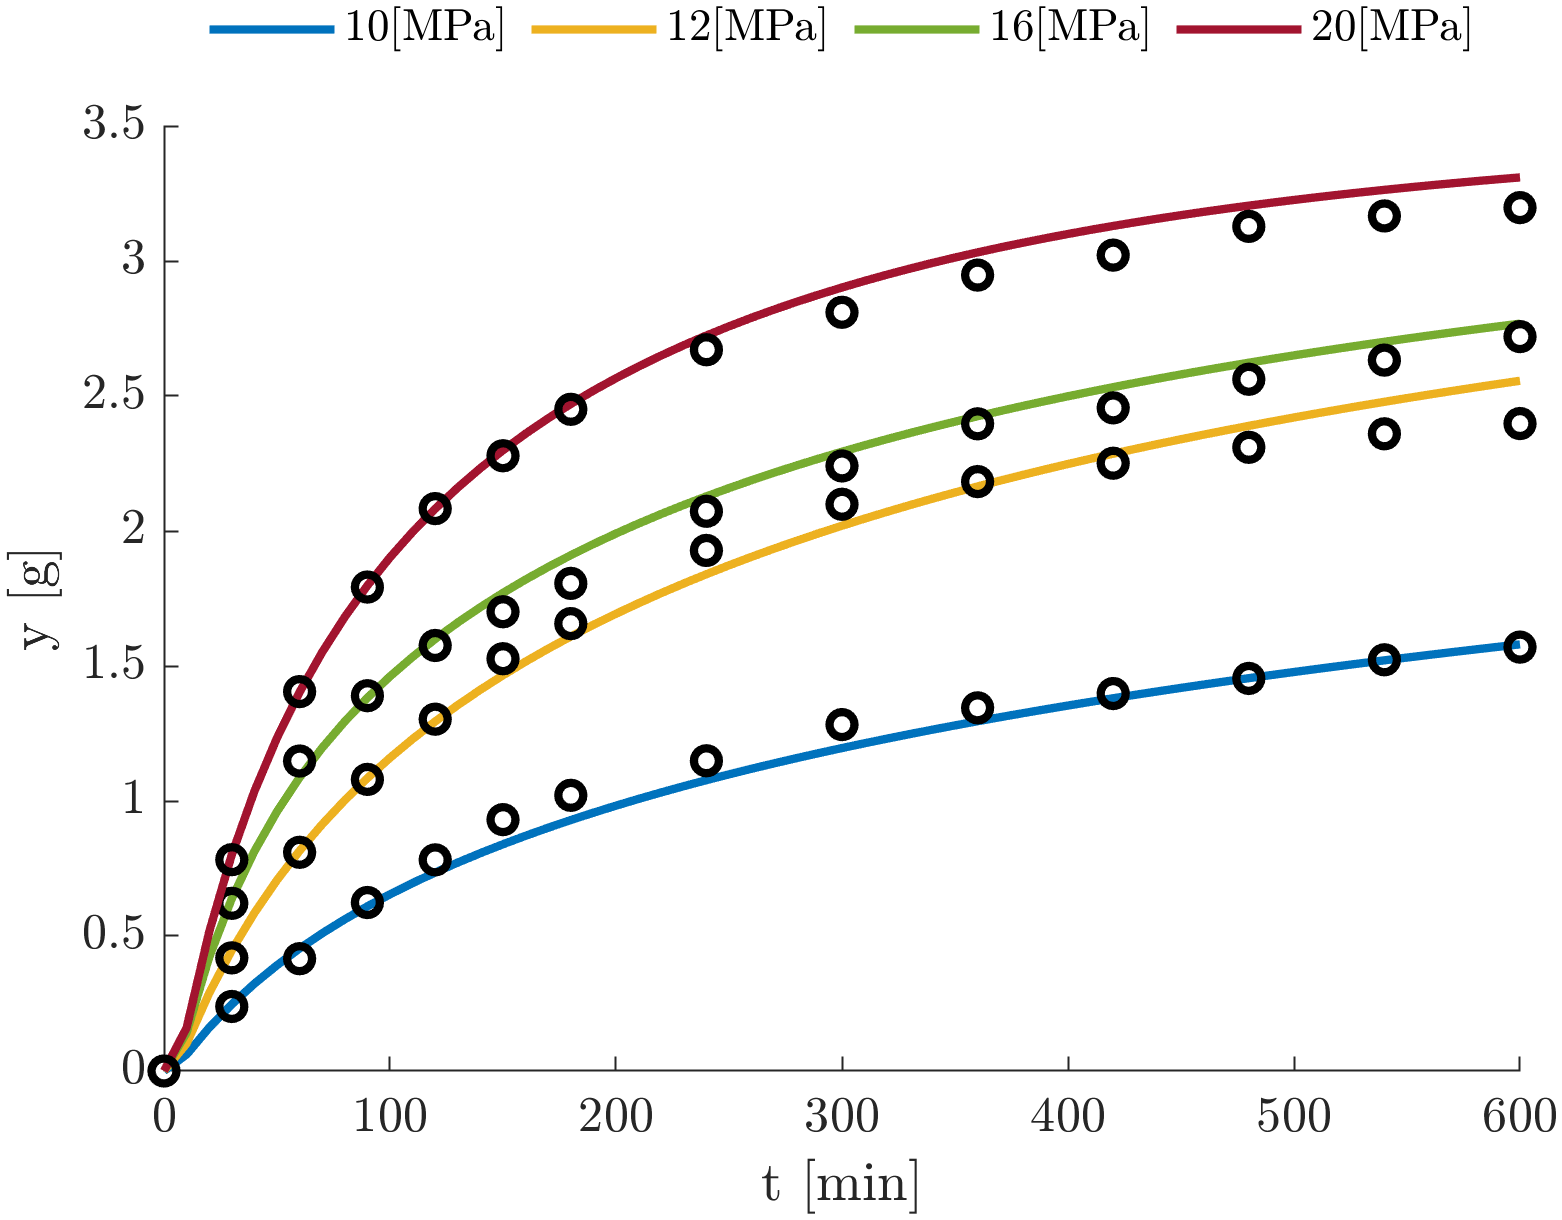
\includegraphics[trim = 0.0cm 0.0cm 0.0cm 0.0cm,clip, width=\columnwidth]{/Results_estimation/Fit_Di_Gamma_1_4.png}
			\caption{Results of parameter estimation for experiments at $6.67\times 10^{-5}$ [kg/s] and temperature of 313 [K]}
			\label{fig: Fit_1_4_Di_Gamma}
		\end{subfigure}
		\hfill
		\begin{subfigure}[b]{\columnwidth}
			\centering
			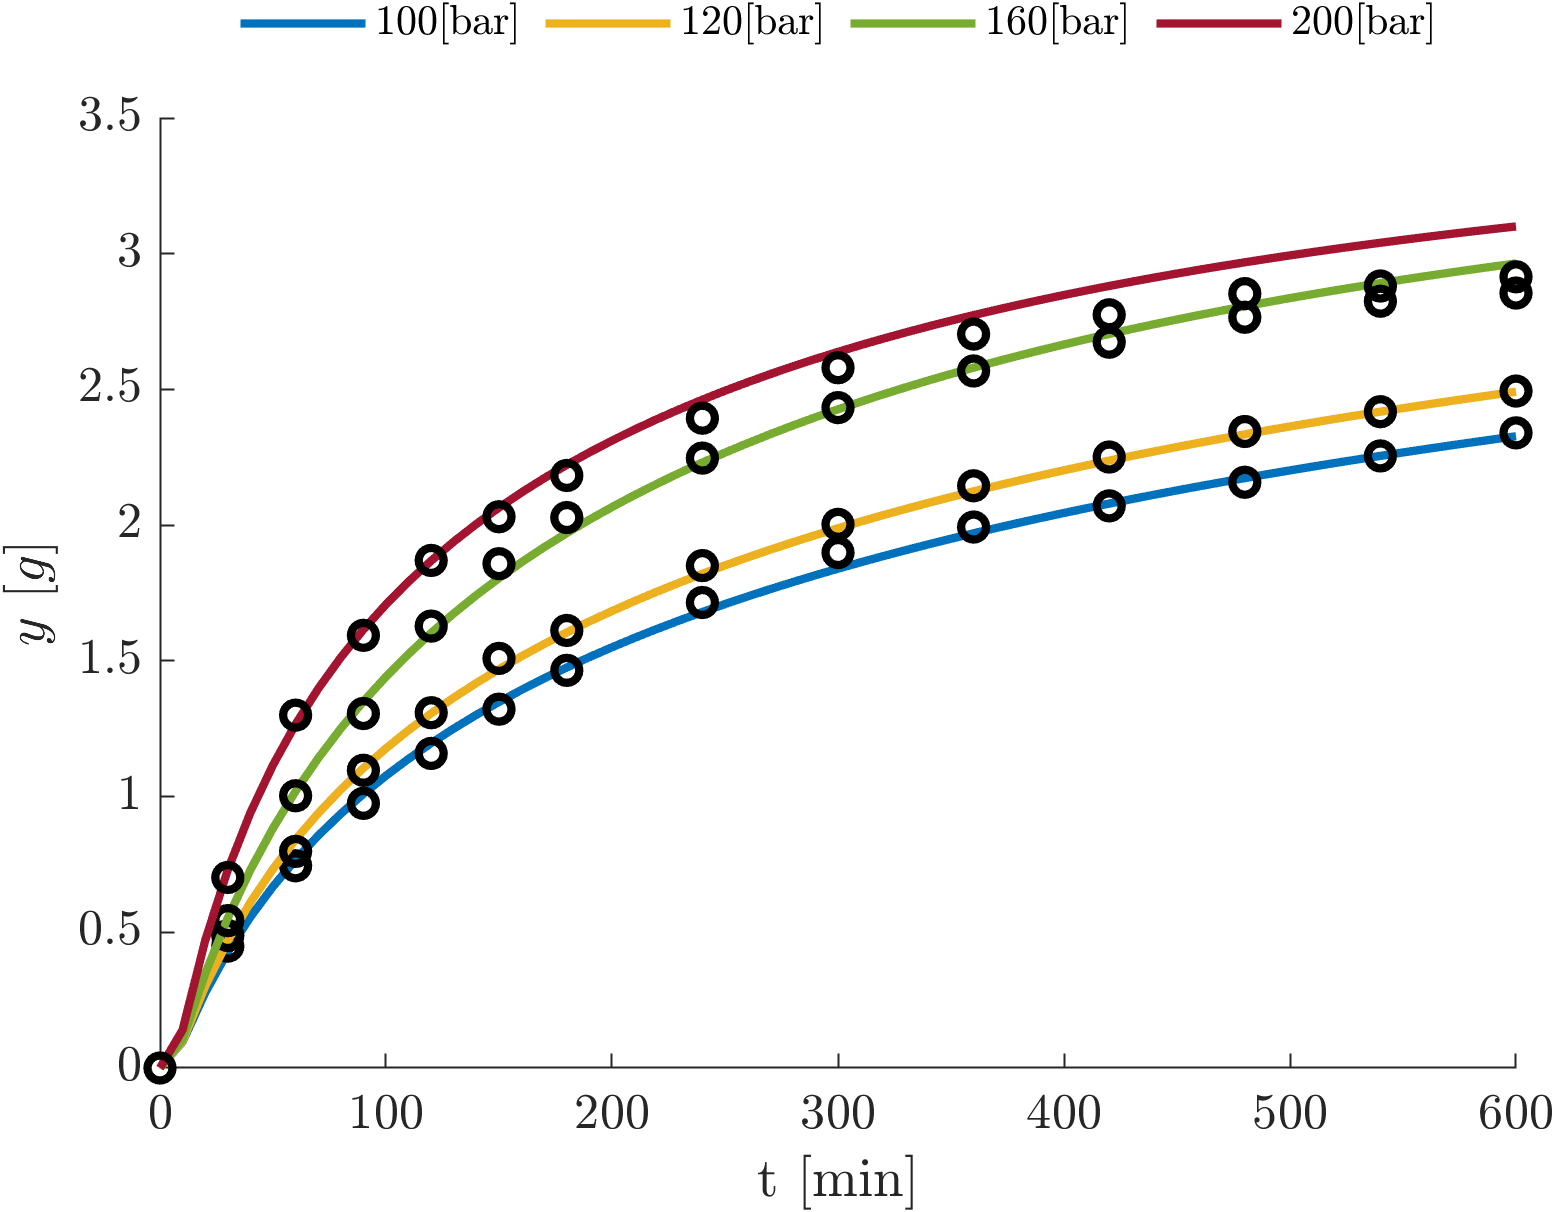
\includegraphics[trim = 0.0cm 0.0cm 0.0cm 0.0cm,clip, width=\columnwidth]{/Results_estimation/Fit_Di_Gamma_5_8.png}
			\caption{Results of parameter estimation for experiments at $6.67\times 10^{-5}$ [kg/s] and temperature of 303 [K]}
			\label{fig: Fit_5_8_Di_Gamma}
		\end{subfigure}
		\hfil
		\begin{subfigure}[b]{\columnwidth}
			\centering
			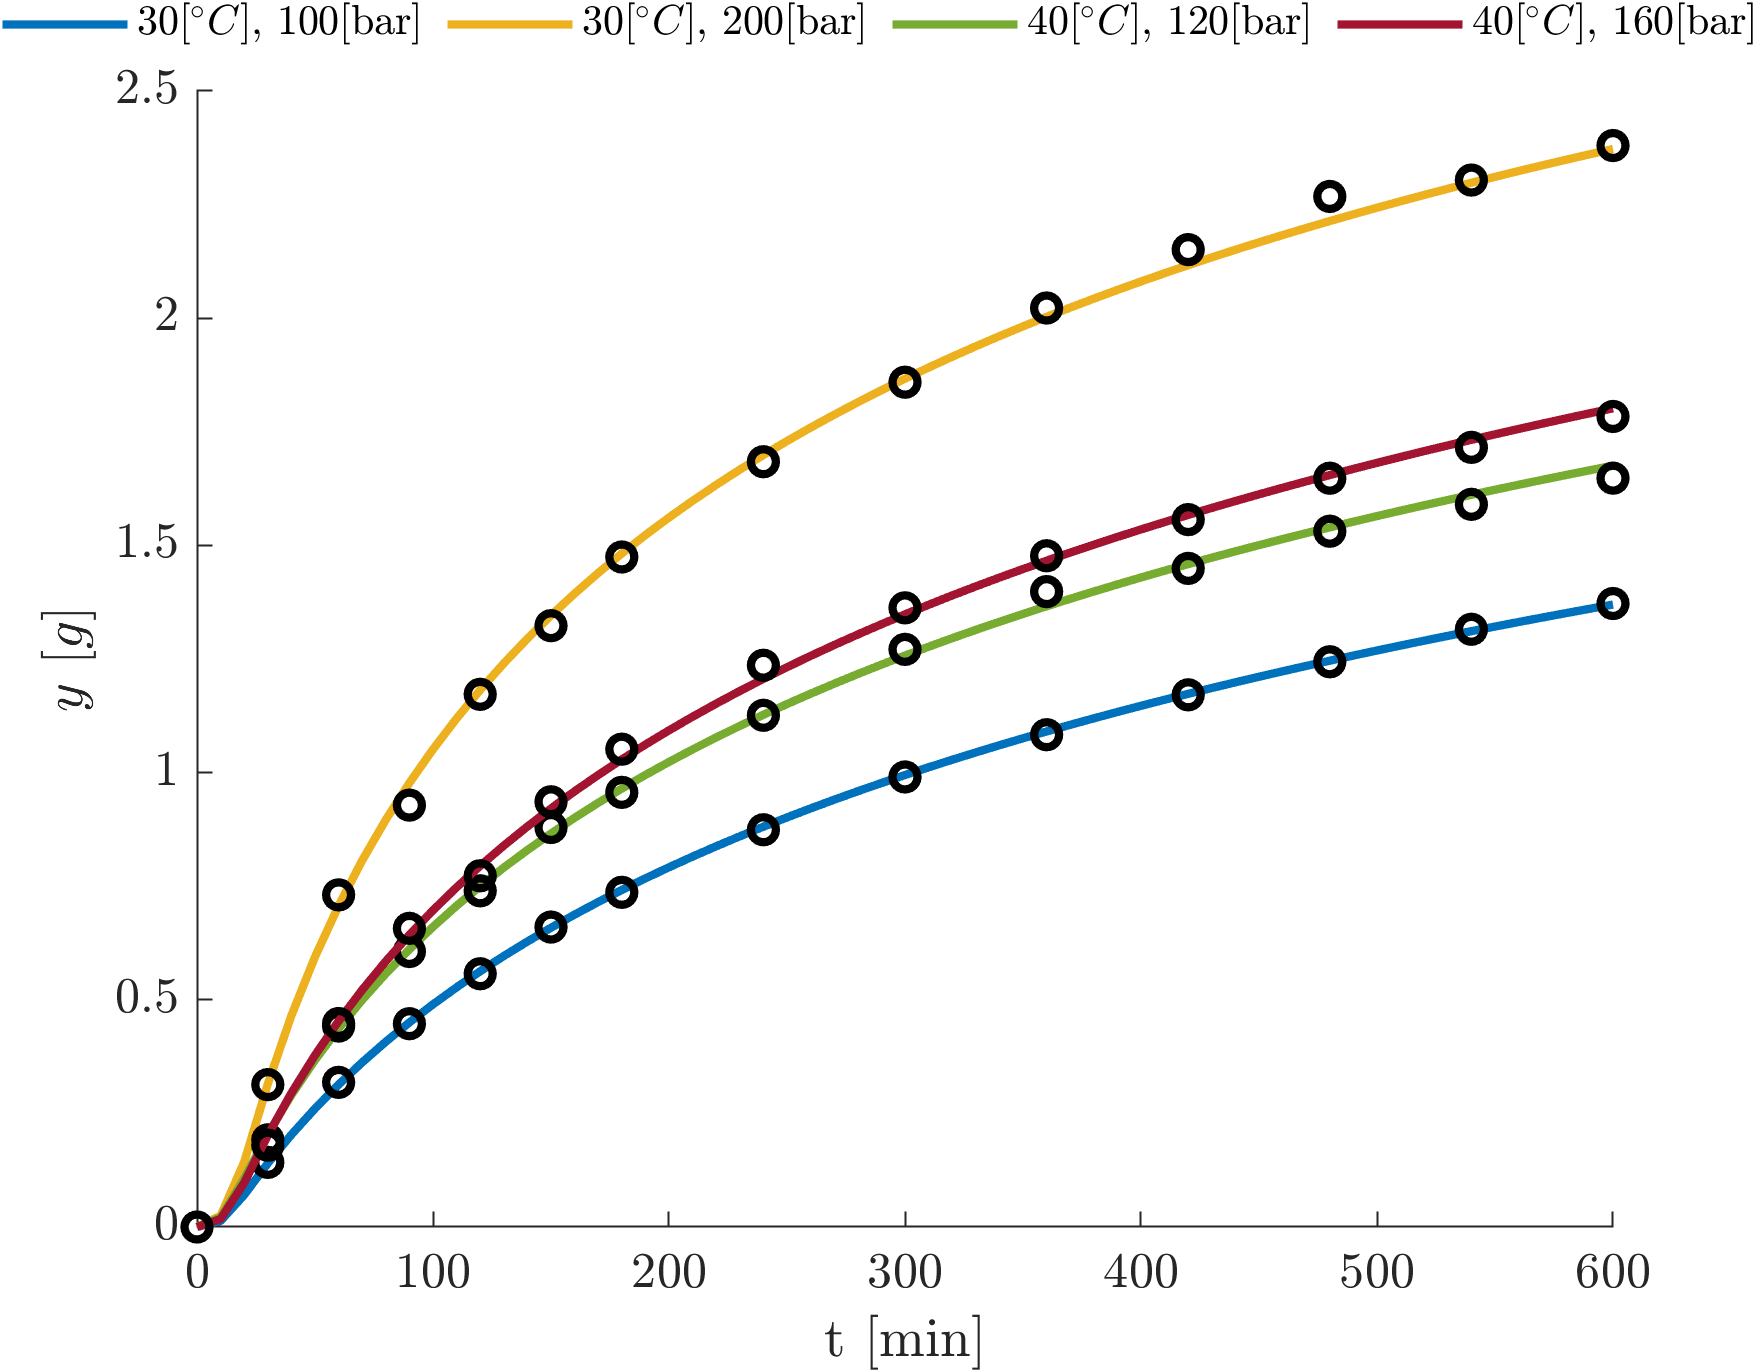
\includegraphics[trim = 0.0cm 0.0cm 0.0cm 0.0cm,clip, width=\columnwidth]{/Results_estimation/Fit_Di_Gamma_9_12.png}
			\caption{Results of parameter estimation for experiments at $3.33\times 10^{-5}$ [kg/s]}
			\label{fig: Fit_9_12_Di_Gamma}
		\end{subfigure}
		\caption{Parameter estimation results}
		\label{fig: Fit_Di_Gamma}
	\end{figure}
		
	The results from the parameter estimation are further combined to obtain general correlations, which can be used for modelling of the extraction process at dynamically changing operating conditions. The traditional approach for finding correlations by combining Reynolds, Schmidt and Sherwood numbers is not used here because the axial diffusion rate was considered to be negligible. The proposed correlations shows linear trend between obtained parameters and the Reynolds number $\left(Re = \frac{\rho_f u d_p}{\mu}\right)$, as shown in Figure \ref{fig: Correlations}.
	
	\begin{figure}
		\centering
		\begin{subfigure}[b]{\columnwidth}
			\centering
			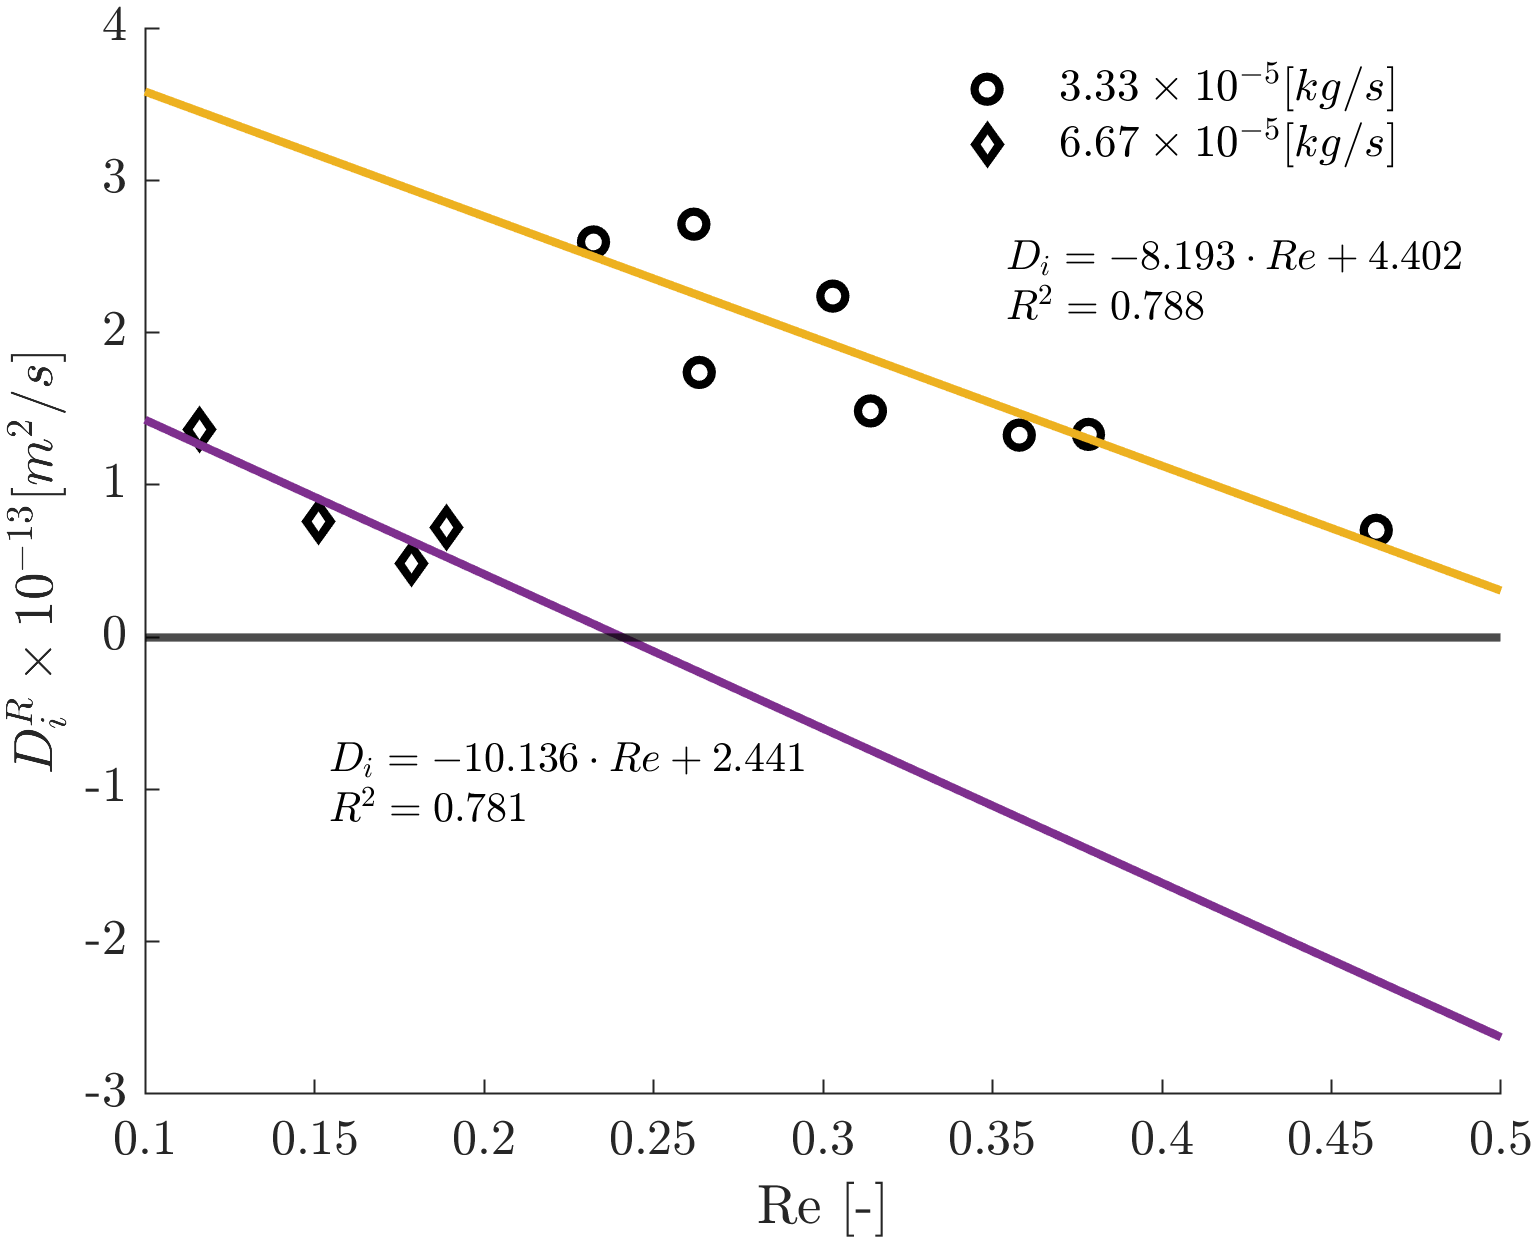
\includegraphics[trim = 0.0cm 0.0cm 0.0cm 0.0cm,clip, width=\columnwidth]{/Results_estimation/Correlation_Di_Re.png}
			\caption{Linear regression $D_i^R$}
			\label{fig: Correlations_Di_Re}
		\end{subfigure}
		\hfill
		\begin{subfigure}[b]{\columnwidth}
			\centering
			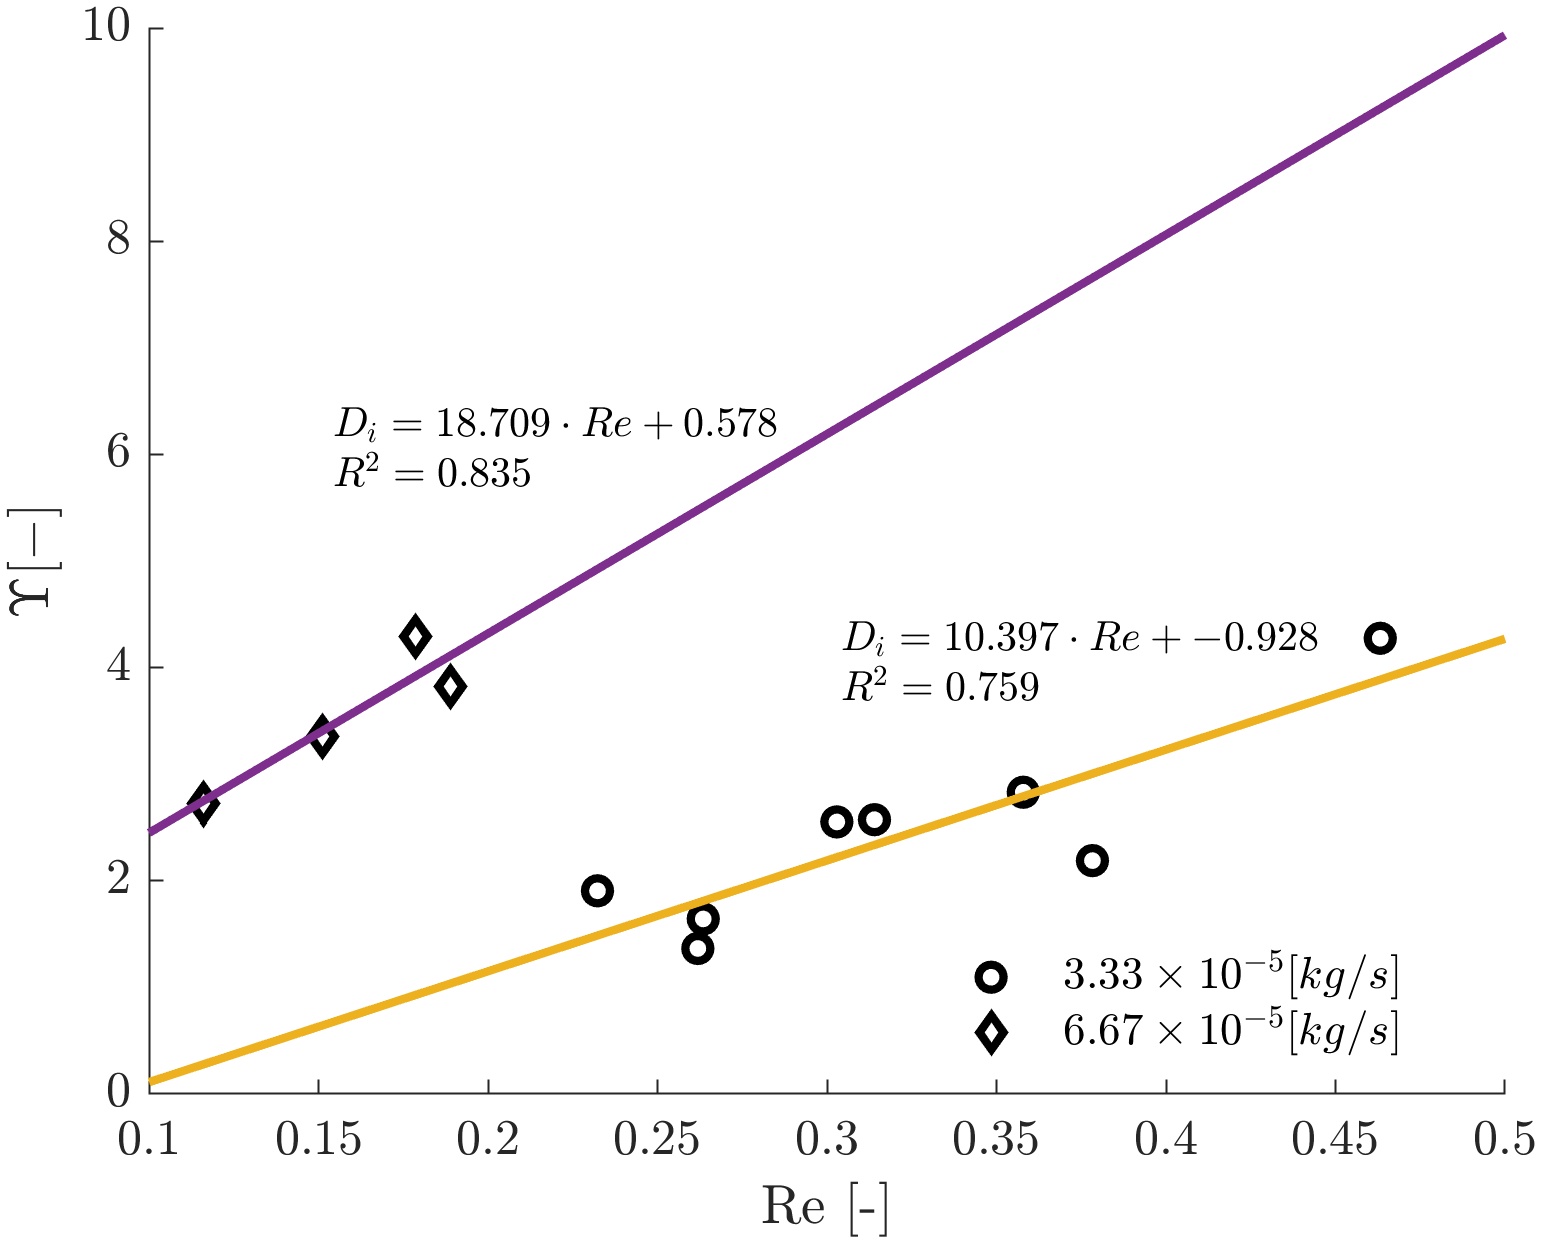
\includegraphics[trim = 0.0cm 0.0cm 0.0cm 0.0cm,clip, width=\columnwidth]{/Results_estimation/Correlation_Gamma_Re.png}
			\caption{Linear regression $\Upsilon$}
			\label{fig: Correlations_Gamma_Re}
		\end{subfigure}
		\caption{Parameter estimation results}
		\label{fig: Correlations}
	\end{figure}
	
\end{document}